\documentclass[a4paper,twocolumn]{article}


\usepackage[sc]{mathpazo} % Use the Palatino font
\usepackage[T1]{fontenc} % Use 8-bit encoding that has 256 glyphs
\usepackage[utf8]{inputenc} % Use utf-8 as encoding
\linespread{1.05} % Line spacing - Palatino needs more space between lines
\usepackage{microtype} % Slightly tweak font spacing for aesthetics
\usepackage{graphicx}

\usepackage[spanish]{babel} % Language hyphenation and typographical rules
%\usepackage[galician]{babel} % Change to this if using galician

\usepackage[hmarginratio=1:1,top=32mm,columnsep=20pt]{geometry} % Document margins
\usepackage[hang, small,labelfont=bf,up,textfont=it,up]{caption} % Custom captions under/above floats in tables or figures
\usepackage{booktabs} % Horizontal rules in tables

\usepackage{enumitem} % Customized lists
\setlist[itemize]{noitemsep} % Make itemize lists more compact

\usepackage{abstract} % Allows abstract customization
\renewcommand{\abstractnamefont}{\normalfont\bfseries} % Set the "Abstract" text to bold
\renewcommand{\abstracttextfont}{\normalfont\small\itshape} % Set the abstract itself to small italic text

\usepackage{titlesec} % Allows customization of titles
\renewcommand\thesection{\Roman{section}} % Roman numerals for the sections
\renewcommand\thesubsection{\Alph{subsection}} % roman numerals for subsections
\titleformat{\section}[block]{\large\scshape\centering}{\thesection.}{1em}{} % Change the look of the section titles
\titleformat{\subsection}[block]{\large}{\thesubsection.}{1em}{} % Change the look of the section titles

\usepackage{fancyhdr} % Headers and footers
\pagestyle{fancy} % All pages have headers and footers
\fancyhead{} % Blank out the default header
\fancyfoot{} % Blank out the default footer
%\fancyhead[C]{Running title $\bullet$ May 2016 $\bullet$ Vol. XXI, No. 1} % Custom header text
\fancyfoot[C]{\thepage} % Custom footer text

\usepackage{titling} % Customizing the title section

\usepackage{hyperref} % For hyperlinks in the PDF

\usepackage{listings}
\usepackage{xcolor}

\usepackage{float}

\usepackage{amsmath}

% Configuración de los listings para mostrar código
\lstset{
    language=C,                % Lenguaje de programación
    basicstyle=\small\ttfamily, % Estilo básico y tamaño de fuente
    keywordstyle=\color{blue}, % Estilo de las palabras clave
    stringstyle=\color{red},   % Estilo de las cadenas de texto
    commentstyle=\color{purple},% Estilo de los comentarios
    morecomment=[l][\color{magenta}]{\#},  % Estilo de los preprocesadores
    breaklines=true,           % Permite que las líneas se partan
    breakatwhitespace=true,    % Los cortes de línea ocurren en los espacios en blanco
    tabsize=4,                 % Tamaño de tabulación
    showstringspaces=false,    % No muestra espacios especiales en las cadenas
    frame=single,              % Añade un marco alrededor del código
    numbers=left,              % Números de línea a la izquierda
    numberstyle=\small,        % Tamaño de fuente de los números de línea
    captionpos=b,              % Posición del título en la parte inferior
    escapeinside={(*@}{@*)}    % Permite añadir LaTeX dentro del código
}

%----------------------------------------------------------------------------------------
%	TITLE SECTION
%----------------------------------------------------------------------------------------

\setlength{\droptitle}{-4\baselineskip} % Move the title up

\pretitle{\begin{center}\huge\bfseries} % Article title formatting
	\posttitle{\end{center}} % Article title closing formatting

\title{Desenrolle de lazos internos con optimización de operaciones de reducción} % Article title

\date{\today} % Leave empty to omit a date
\renewcommand{\maketitlehookd}{%
	\begin{abstract}
		\noindent En este informe se abordará el tema del desenrrolle de lazos y como afecta su produndidad en términos de tiempo de ejecución del programa.  \\\mbox{}\\
		 \textbf{\textit{Palabras clave}: bucles, lazos, unrolling, desenrollamiento, optimización\ldots}
	\end{abstract}
}
%----------------------------------------------------------------------------------------

\begin{document}
	
	% Print the title
	\maketitle
	
	%----------------------------------------------------------------------------------------
	%	ARTICLE CONTENTS
	%----------------------------------------------------------------------------------------
	
	\section{Introducción}

        En el presente informe se describe una serie de experimentos diseñados para estudiar la técnica denominada desenrollamiento de lazos, en el contexto de operaciones de reducción, y su profundidad. Con su profundidad nos referimos a la cantidad de veces que se ejecuta el cuerpo del bucle en cada iteración.
        
        Para el estudio, se realizarán varios programas breves escritos en el lenguaje de bajo nivel C, ejecutados en un sistema operativo UNIX. Para la medición de los tiempos de ejecución de los bucles for se utilizará la librería \textit{sys/time.h}.

 
%	Introducción al problema tratado, incluyendo las referencias  necesarias. Por ejemplo: ``Este trabajo se basa en los estudios teóricos realizados en~\cite{Intel:2005} y \cite{spec}". En este apartado se plantean el problema a resolver, objetivos a alcanzar y metodología seguida para alcanzarlos.
	
%	Es una introducción al problema, no se desarrollarán los contenidos aquí. 
	
%	La introducción termina indicando en pocas palabras de qué secciones consta el resto del documento y de qué trata cada una. Se mencionan todas las secciones salvo la de referencias (bibliografía). 

	%------------------------------------------------
	
%-------------------------------------------

\section{Descripción de la técnica analizada: Loop Unrolling}

El desenrollamiento de lazos (loop unrollig en inglés), es una técnica que consiste en intentar minimizar el coste temporal de un bucle o lazo, mediante la reducción del número de iteraciones del mismo. 

Básicamente lo que hacemos en esta es la de eliminar o reducir las iteraciones necesarias para realizar una operación, reduciendo así el tiempo de ejecución de la misma. 

Un sencillo ejemplo es el siguiente:

\begin{lstlisting}[caption={Bucle sin desenrollar},label={lst:codigoC}]
	// This program does not uses loop unrolling. 
	#include<stdio.h> 
	
	int main(void) 
	{ 
		for (int i=0; i<5; i++) 
			printf("Hello\n"); //print hello 5 times 
	
		return 0; 
	}
\end{lstlisting}

\begin{lstlisting}[caption={Bucle aplicando la técnica},label={lst:codigoC}]
	// This program uses loop unrolling. 
	#include<stdio.h> 
	
	int main(void) 
	{ 
		// unrolled the for loop in program 1 
		printf("Hello\n"); 
		printf("Hello\n"); 
		printf("Hello\n"); 
		printf("Hello\n"); 
		printf("Hello\n"); 
	
		return 0; 
	} 
\end{lstlisting}

Ambos programas [1] nos muestran un sencillo ejemplo de la aplicación de esta técnica, pudiendo observar en el segundo caso se ha eliminado por completo el bucle, reduciendo así el tiempo de ejecución del programa, debido a que dentro del bucle es necesario hacer una comprobación del índice, lo que ralentiza el código. 

Otra manera diferente, para lazos donde eliminar el bucle por completo no es posible, se pueden reducir el número de iteraciones realizando varias operaciones en una sola iteración. 

Por ejemplo: imaginemos que tenemos un bucle el cual almacena en una variable el sumatorio de los números del 1 al 10. En un bucle sin desenrollamiento tendríamos que realizar 10 iteraciones, donde en cada una realizamos una operación. Sin embargo, podemos reducir el número de iteraciones a la mitad si en vez de sumar de uno en uno, sumamos de dos en dos, y a su vez podríamos reducirlo a 2 iteraciones si sumamos de 5 en 5. Esto es la otra manera (y que a su vez veremos posteriormente en los experimentos) de aplicar la técnica de desenrollamiento de lazos.

\section{Beneficios y desventajas}

Como casi cualquier herramienta que podamos utilizar, esta técnica conlleva una serie de ventajas y desventajas. Algunas de las ventajas que podemos encontrar son:

\textbf{Ventajas:}
\begin{enumerate}
	\item \textbf{Reducción de la Sobrecarga de Ciclos de Bucle:} En cualquier sistema, reducir la frecuencia con la que se evalúan las condiciones del bucle y se actualizan las variables de control puede mejorar el rendimiento al disminuir la sobrecarga general del bucle.
	\item \textbf{Incremento en el Paralelismo:} En sistemas con capacidades de procesamiento paralelo, desenrollar bucles puede permitir que múltiples operaciones se ejecuten al mismo tiempo, mejorando el uso del paralelismo inherente al hardware.
	\item \textbf{Mejor Uso de las Unidades de Procesamiento:} Al desenrollar un bucle, se pueden realizar más cálculos por cada entrada al bucle, lo cual puede ser eficiente en términos de aprovechamiento del tiempo de CPU y la ejecución en pipelining.
    \item \textbf{Reducción en el Tiempo de Ciclo de Reloj:} A medida que se desenrollan los bucles y el área utilizada se reduce inicialmente, puede resultar en un decremento en el tiempo de ciclo de reloj, lo cual potencialmente incrementa la frecuencia de operación y por ende la velocidad de procesamiento.
    \item \textbf{Disminución en el Uso del Área de FPGA (Field Programmable Gate Array) en Ciertos Casos:} Inicialmente, el desenrollamiento puede llevar a una reducción en el área utilizada, lo que es beneficioso cuando el área es una limitante crítica en el diseño del sistema.
\end{enumerate}

\textbf{Desventajas:}
\begin{enumerate}
	\item \textbf{Aumento del Tamaño del Código:} Desenrollar bucles aumenta la cantidad de código que se ejecuta, lo cual puede llevar a un mayor uso de la memoria de instrucciones y potencialmente a un caché de instrucciones más ocupado.
	\item \textbf{Complicaciones en la Gestión de la Memoria:} El aumento en la cantidad de operaciones ejecutadas simultáneamente puede hacer que la gestión de memoria sea más compleja y puede presionar al ancho de banda de memoria disponible.
	\item \textbf{Limitaciones por Dependencias de Datos:} Si existen dependencias de datos dentro de las iteraciones de un bucle, el desenrollamiento puede no ser aplicable sin modificar significativamente el algoritmo o puede llevar a la ejecución ineficiente debido a la espera de datos.
	\item \textbf{Inflexibilidad en la Modificación del Código:} El código desenrollado es menos flexible para modificaciones futuras o ajustes de parámetros del bucle, ya que cualquier cambio requiere más esfuerzo para actualizar todas las instancias desenrolladas del bucle.
\end{enumerate}

Por tanto, viendo las ventajas y las desventajas, el programador deberá valorar si aplicar esta técnica en su código, ya que aunque puede mejorar el rendimiento, también puede conllevar una serie de problemas.

\subsection{Experimentos}

Para la realización de los experimentos hay que tener en cuenta un factor fundamental, y es referido al tamaño del array. Este debe ser divisible entre el número de desenrolles que queramos hacer, de tal manera que que no se produzca ningún error de acceder a posiciones que no existen.

Por tanto, y teniendo en cuenta lo anterior lo que hacemos es utilizar los múltiplos de 2 desde el 16 hasta el 8192, para que no haya problemas de acceso a memoria. A su vez ponemos un número de iteraciones suficientemente alto para que se pueda apreciar la diferencia entre los bucles desenrollados y los que no lo están. En este caso, hemos puesto 2 000 000 iteraciones.

También es destacable que utilizamos factores de desenrollamiento que sean potencias de 2 para que se alineen mejor con los tamaños de los resigtros y la arquitecutra del hardware.

\subsubsection{Desenrolle de tamaño 4}

Para empezar con los experimentos, haremos un desenrolle de tamaño, es decir, que en cada iteración del bucle se realizarán 4 operaciones. Para esto, mediremos el tiempo de ejecución de un bucle normal y de uno desenrollado y los compararemos.

De los resultados temporales obtenemos la siguiente gráfica:

\begin{figure}[H]
	\centering
	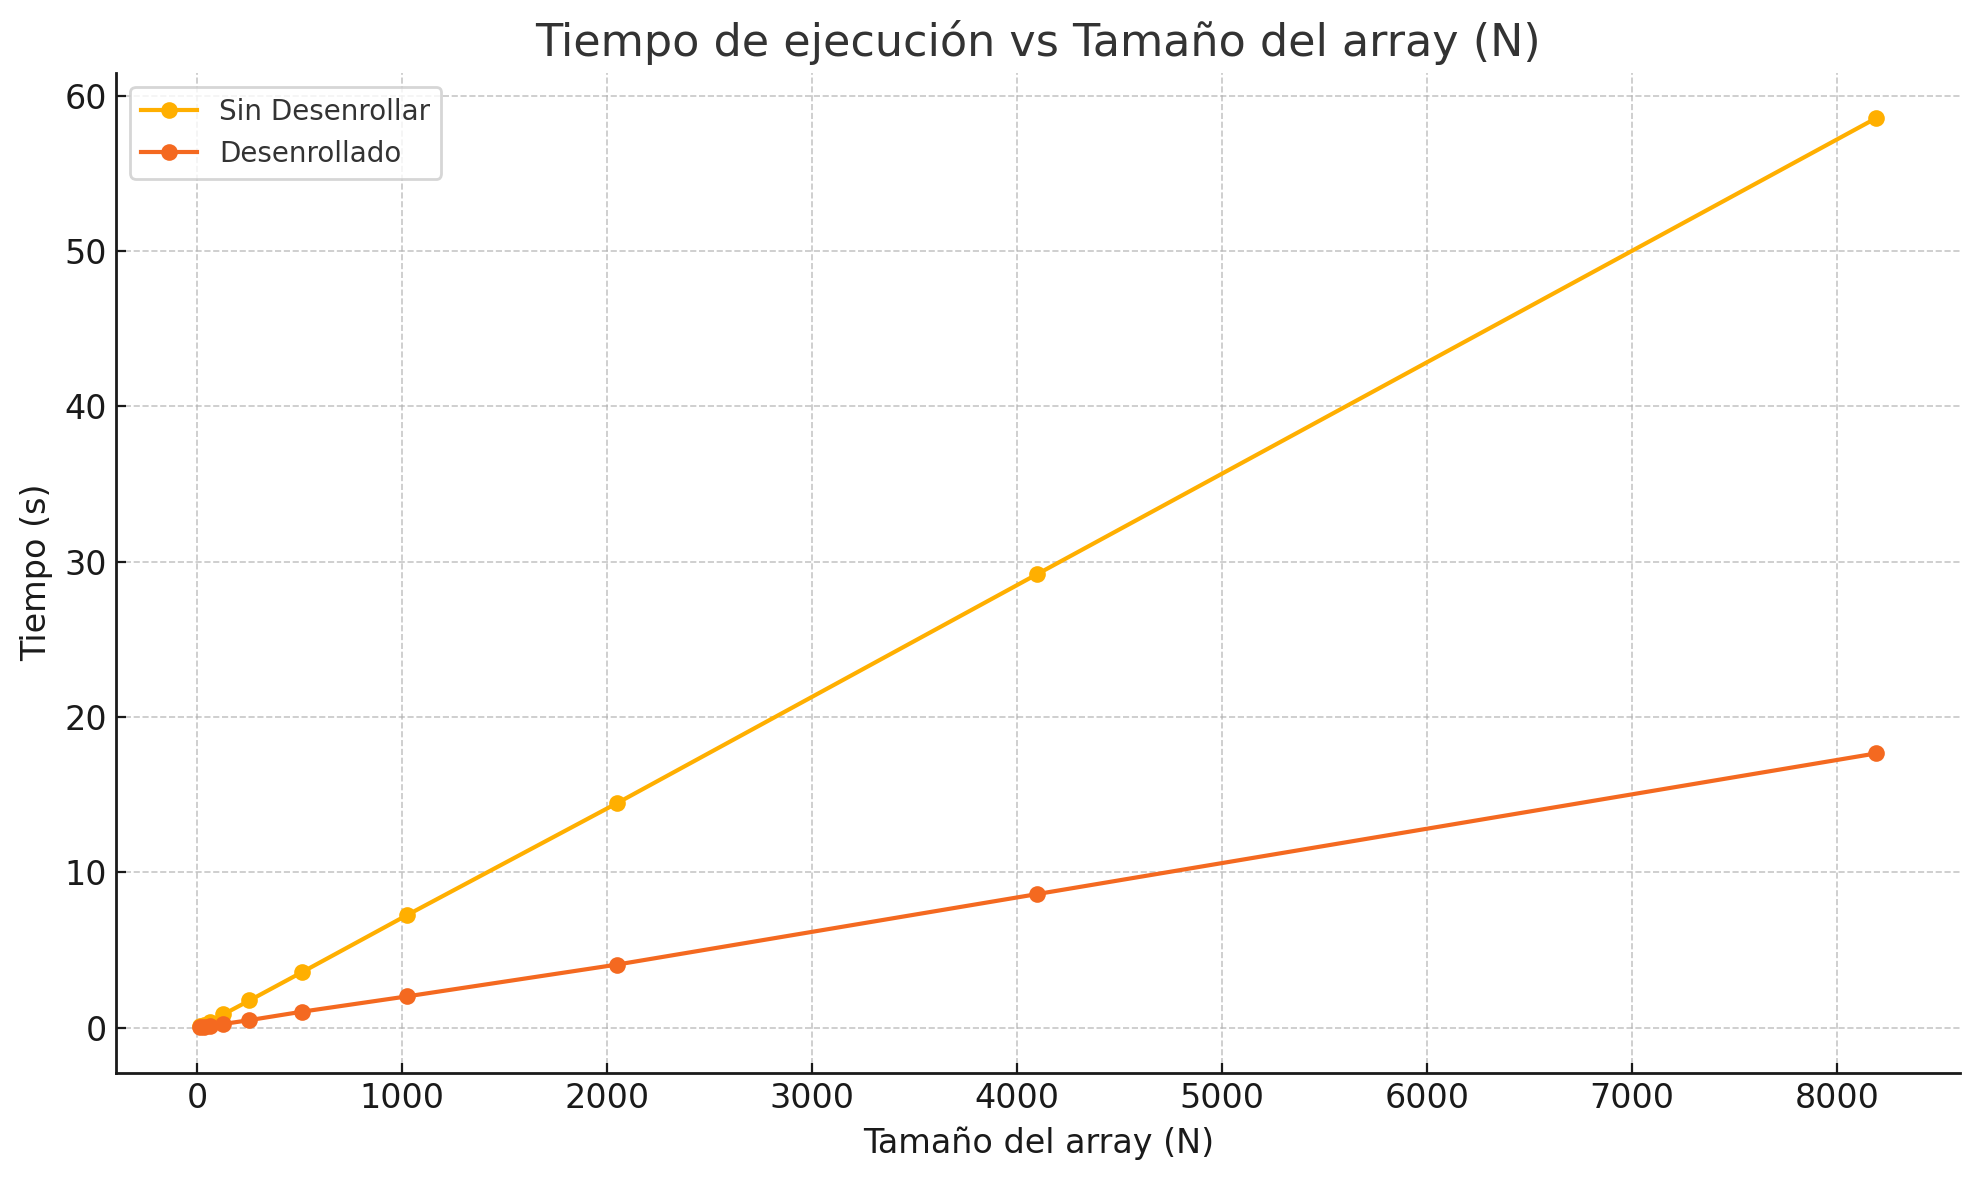
\includegraphics[width=\columnwidth]{4.png}
	\caption{Tiempos de ejecución para un bucle desenrollado de tamaño 4}
	\label{fig:times}
\end{figure}

Como podemos comprobar en la gráfica, el desenrolle de lazos mejora el tiempo de ejecución del programa, y a medida que incremental el tamaño del array, la diferencia entre ambos bucles se hace más notable, como comprobamos en la siguiente gráfica donde medimos el porcentaje de memoria:

\begin{figure}[H]
	\centering
	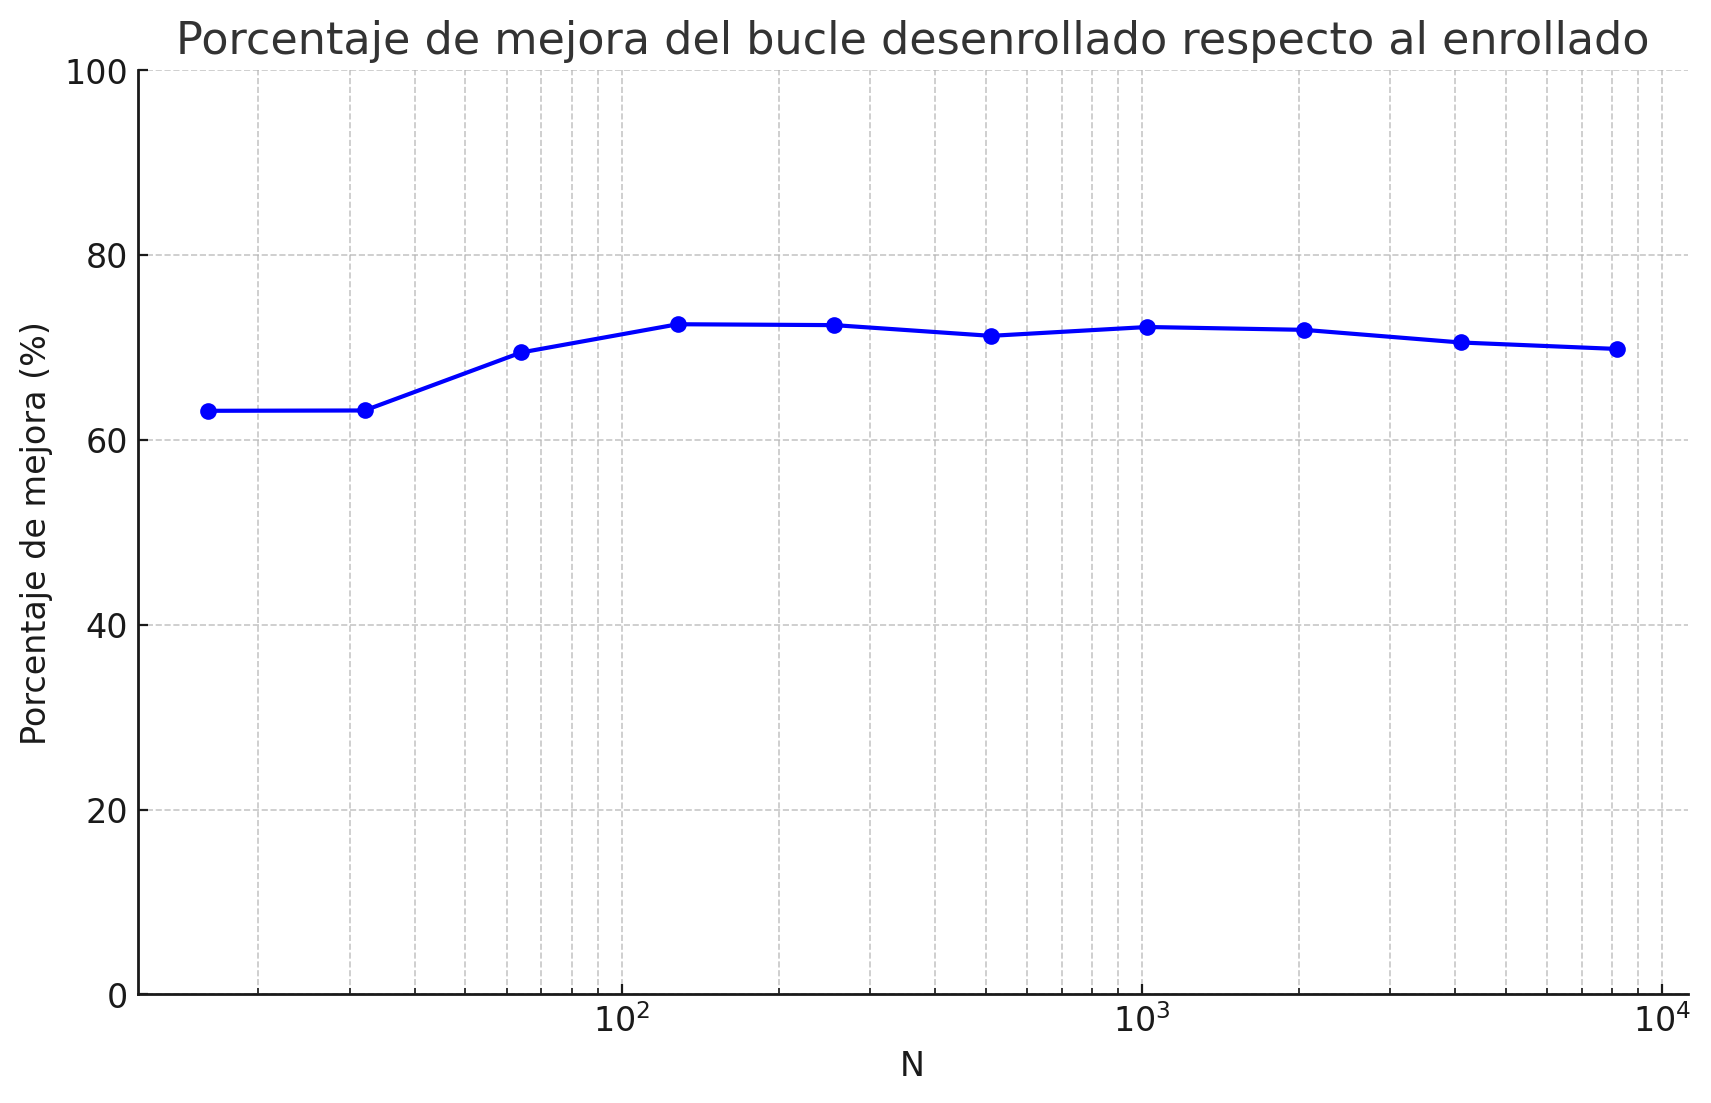
\includegraphics[width=\columnwidth]{4Histograma.png}
	\caption{Porcentaje de mejora del bucle desenrollado respecto al enrollado}
	\label{fig:times}
\end{figure}

Por tanto podemos concluir que en térmimos de eficiencia temporal, el desenrolle de lazos mejora la eficiencia temporal del programa, y que a mayor el tamaño del array, mayor será la diferencia entre ambos bucles.

\subsubsection{Comparación de los desenrolles}

Puesto que en los dos experimentos anteriores sacamos las mismas conclusiones (es decir, que el desenrolle mejora la eficiencia temporal), vamos a comparar los desenrolles entre sí, así como añadir para d = 8 y 16.

La gráfica es la siguiente: 

\begin{figure}[H]
	\centering
	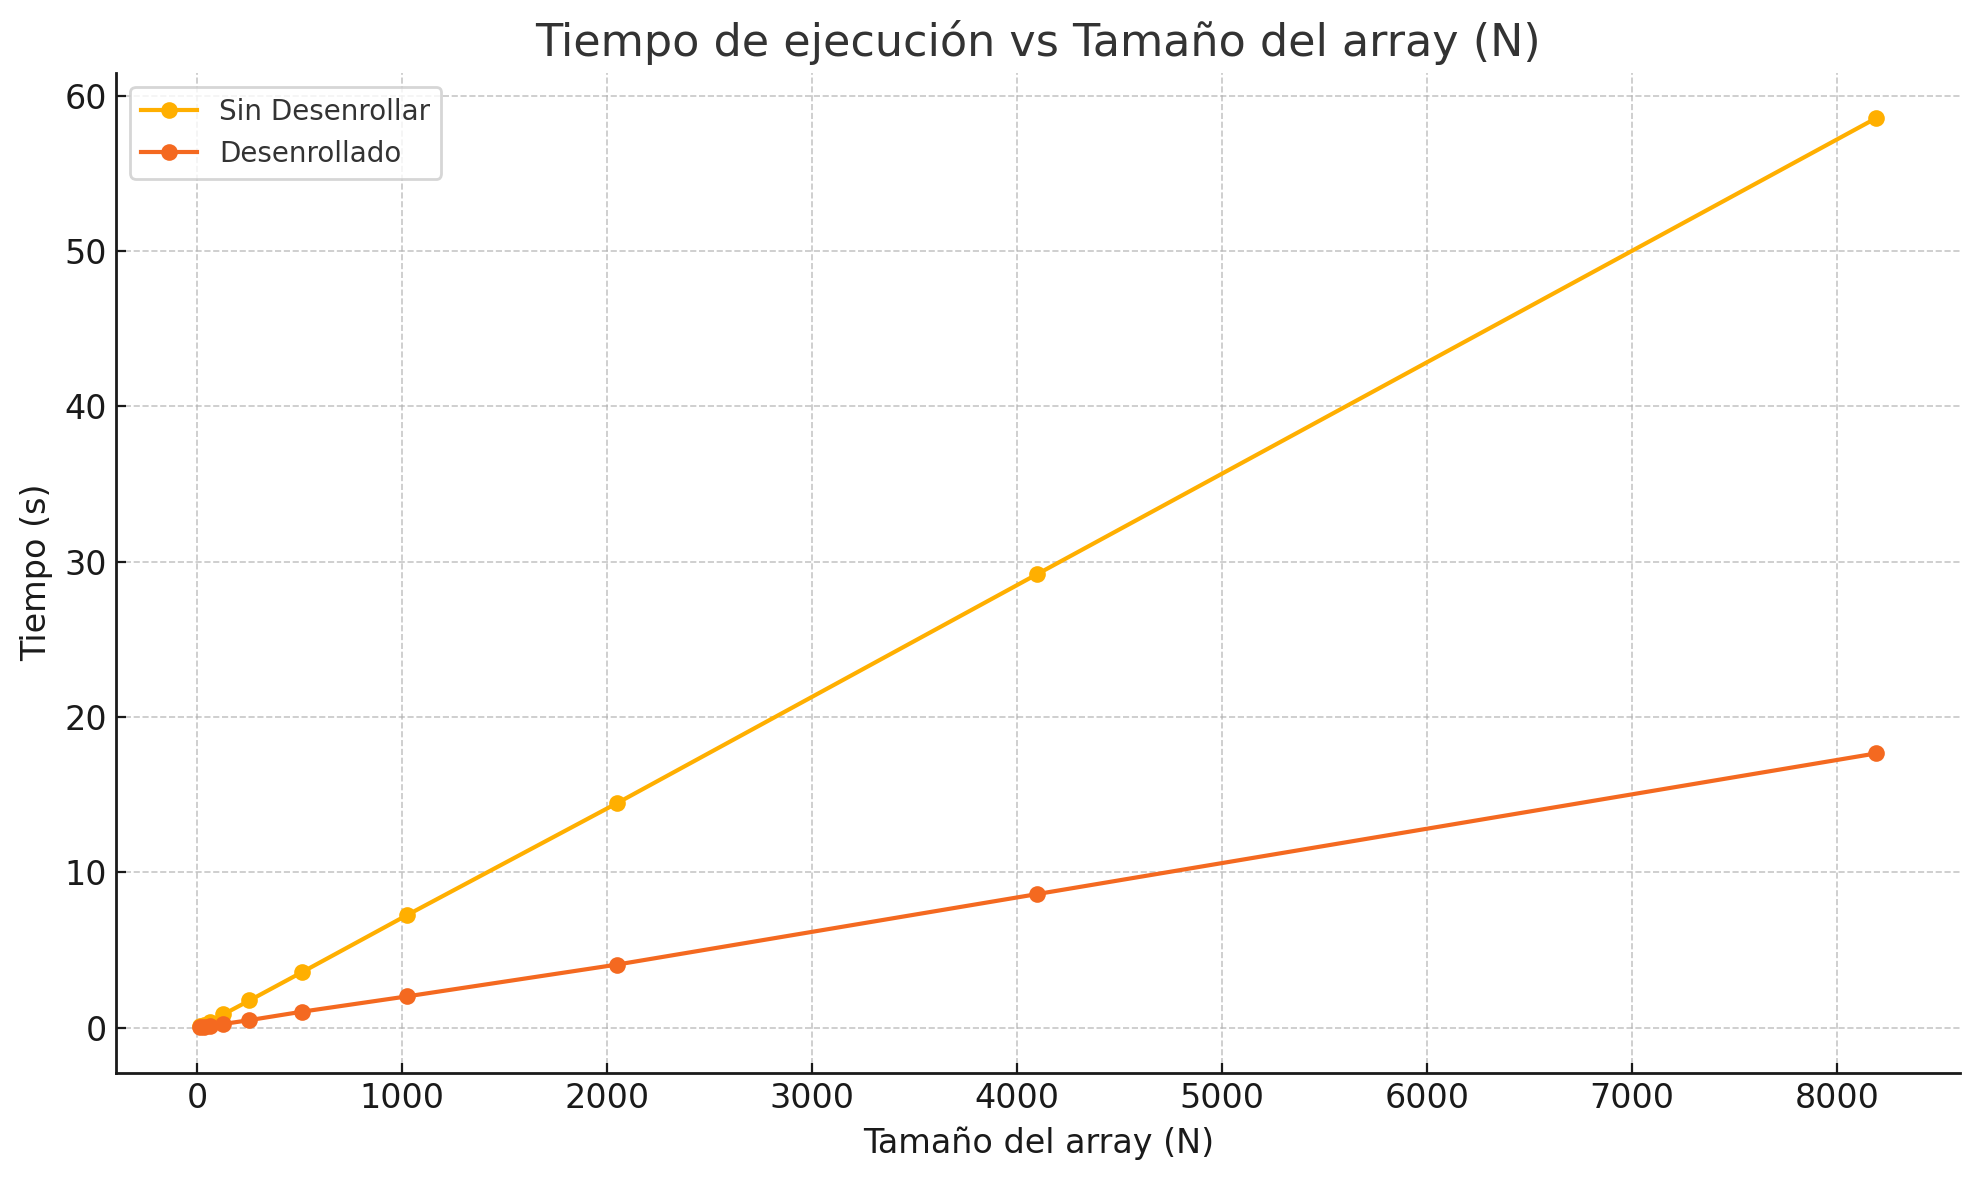
\includegraphics[width=\columnwidth]{4.png}
	\caption{Tiempos de ejecución para un bucle desenrollado de tamaño 4}
	\label{fig:times}
\end{figure}


\section{Resultados}
\begin{figure}[h]
    \centering
    \includegraphics[width=0.5\textwidth]{execution_times.png}
    \caption{Tiempos de ejecución para diferentes valores de `d`}
    \label{fig:times}
\end{figure}

\section{Discusión}
\begin{itemize}
    \item ¿Qué valor de `d` proporciona el mejor rendimiento?
    \item ¿Hay un punto en el que el rendimiento empeora?
    \item ¿Cuáles podrían ser las causas?
\end{itemize}

\section{Conclusiones}
En este informe, se estudió el desenrolle de lazos con diferentes profundidades y se analizaron los efectos en el tiempo de ejecución. Los resultados mostraron que \ldots

%----------------------------------------------------------------------------------------
%	Referencias
%----------------------------------------------------------------------------------------
	
\begin{thebibliography}{99} % Bibliografía - alternativamente, se recomienda el uso de bibtex o biblatex

    \bibitem[1]{LoopUnrollingGeeksforGeeks}
    GeeksforGeeks.
    \newblock {\em Loop Unrolling}.
    \newblock \url{https://www.geeksforgeeks.org/loop-unrolling/}, \newblock [online]
    
    \bibitem[2]{Dragomir2009}
    O. S. Dragomir, T. Stefanov, and K. Bertels.
    \newblock Optimal Loop Unrolling and Shifting for Reconfigurable Architectures.
    \newblock {\em ACM Transactions on Reconfigurable Technology and Systems}, Vol. 2, No. 4, Article 25, September 2009, 24 pages.
    \newblock DOI = 10.1145/1575779.1575785.
    \newblock \url{http://doi.acm.org/10.1145/1575779.1575785}, \newblock [online]

    \bibitem[3]{Buyukkurt2004}
    Betul Buyukkurt, Zhi Guo, and Walid A. Najjar.
    \newblock {\em Impact of Loop Unrolling on Area, Throughput and Clock Frequency in ROCCC: C to VHDL Compiler for FPGAs}.
    \newblock Department of Computer Science and Engineering, University of California - Riverside, Riverside, CA 92507, USA.
    
\end{thebibliography}


	
	%----------------------------------------------------------------------------------------
	
\end{document}